\documentclass[12pt]{article}
\usepackage[a4paper, left=2cm, right=2cm, top=2cm, bottom=2cm]{geometry}
\usepackage{fontspec}
\usepackage{booktabs}
\usepackage{amsmath, amsfonts}
\usepackage{graphicx}
\usepackage{circuitikz}
\usepackage{polyglossia}
\usepackage{float}
\setdefaultlanguage{greek}
\setotherlanguage{english}
\setmainfont{Palatino Linotype}
\usepackage{subcaption}
\usepackage{siunitx}
\usepackage{bm}

% This is for code
\usepackage{listings}
\usepackage{xcolor} % Required for custom colors

% This is for CSV
\usepackage{csvsimple-l3}


% Define custom colors
\definecolor{codegreen}{rgb}{0,0.6,0}
\definecolor{codegray}{rgb}{0.5,0.5,0.5}
\definecolor{codepurple}{rgb}{0.58,0,0.82}
\definecolor{backcolour}{rgb}{0.95,0.95,0.92}

% Define a custom style for C code
\lstdefinestyle{CStyle}{
    language=C,
    backgroundcolor=\color{backcolour},   
    commentstyle=\color{codegreen},
    keywordstyle=\color{blue}\bfseries,
    numberstyle=\tiny\color{codegray},
    stringstyle=\color{codepurple},
    basicstyle=\ttfamily\footnotesize,
    breakatwhitespace=false,         
    breaklines=true,                 
    captionpos=b,                    
    keepspaces=true,                 
    numbers=left,                    
    numbersep=5pt,                  
    showspaces=false,                
    showstringspaces=false,
    showtabs=false,                  
    tabsize=4
}

\begin{document}

% --- HEADER START ---
\noindent
\begin{minipage}[t]{\textwidth}
    {\large \textbf{Εθνικό Μετσόβιο Πολυτεχνείο}} \\
    \textbf{Σχολή Ηλεκτρολόγων Μηχανικών και Μηχανικών Υπολογιστών} \\    
    \textbf{Τομέας Τεχνολογίας Πληροφορικής και Υπολογιστών} \\
    Μάθημα: "Σχεδιασμός Ενσωματωμένων Συστημάτων" \\
    Ακαδ. Έτος: 2026-2027
\end{minipage}

\vspace{0.2cm}
\hrule height 1pt
\vspace{1cm}
% --- HEADER END ---


% --- TITLE SECTION ---
\begin{center}
    {\LARGE \textbf{1η Εργαστηριακή Άσκηση}} \\[0.5cm]
    {\large Βελτιστοποίηση Αλγορίθμων για Χαμηλή Κατανάλωση Ενέργειας και Υψηλή Απόδοση}
\end{center}
\vspace{1cm}


% --- AUTHORS SECTION ---
\begin{center}
	\textbf{Αποστολόπουλος Νικόλαος} \\
	(03122614) \\
	\textbf{Γκριμπογιάννης Χαρίλαος} \\
	(03122002)
\end{center}
\vspace{1cm}

% --- ABSTRACT SECTION ---
\begin{center}
    \textbf{\large Περίληψη}
\end{center}

\noindent
Η παρούσα εργασία υλοποιήθηκε στα πλαίσια του μαθήματος "Σχεδιασμός Ενσωματωμένων Συστημάτων" και αφορά ...
\pagebreak

\tableofcontents
\pagebreak

\section{Βελτιστοποίηση της Εφαρμογής tables.c}
Στην παρούσα παράγραφο βελτιστοποιούμε την εφαρμογή tables.c (βλ. Listing \ref{lst:tables}) εκτελούμενη σε δύο διαφορετικές αρχιτεκτονικές x86 με χρήση του προσομοιωτή Gem5. Η πρώτη αρχιτεκτονική που μελετάμε αφορά μια αρχιτεκτονική επεξεργαστή και κύριας μνήμης, ενώ η δεύτερη είναι επαυξημένη με L1 Instruction Cache, L1 Data Cache και L2 Cache. Συγκεκριμένα, μελετάμε την επίδραση της τεχνικής του loop unrolling, καθώς και την επίδραση της ύπαρξης κρυφών μνημών διαφορετικών μεγεθών στον χρόνο εκτέλεσης της εφαρμογής μετρημένο σε κύκλους ρολογιού.

\lstinputlisting[style=CStyle, caption={Source Code (tables.c)}, label={lst:tables}]{tables.c}

\subsection{Σύγκριση Αρχιτεκτονικών}
Αρχικά προσομοιώνουμε την εκτέλεση της εφαρμογής tables.exe σε αρχιτεκτονική που περιλαμβάνει τον επεξεργαστή και την κύρια μνήμη. Η εκτέλεση γίνεται σε 858,490,254 κύκλους. Ύστερα προσομοιώνουμε την εκτέλεση της ίδιας εφαρμογής σε σύστημα που διαθέτει επιπλέον L1 Instruction και L1 Data Caches μεγέθους 8kB και L2 Cache μεγέθους 128kB. Η εφαρμογεί εκτελείται σε 59,829,295 κύκλους. Παρατηρούμε ότι η ενσωμάτωση κρυφών μνημών στο σύστημα μείωσε τον χρόνο εκτέλεσης κατά 798,660,959 κύκλους δίνοντας ένα speedup περίπου 14.35x. Η δραματική αυτή αύξηση της ταχύτητας εκτέλεσης αποδεικνύει έμπρακτα την ανάγκη ύπαρξης των κρυφών μνημών, καθώς χωρίς αυτές κάθε ανάγνωση/εγγραφή που εκτελεί το πρόγραμμα απαιτεί πολύ αργές προσπελάσεις στην κύρια μνήμη.

\subsection{Loop Unrolling}
Αφού αποδείξαμε την ανωτερότητα της αρχιτεκτονικής με κρυφές μνήμες, θα μελετήσουμε πλέον μόνο αυτή την αρχιτεκτονική. Για να ελαττώσουμε περαιτέρω τον χρόνο εκτέλεσης της εφαρμογής, εισάγουμε τη μέθοδο loop unrolling και εξετάζουμε την επίδραση της εφαρμογής της.

Η μέθοδος loop unrolling είναι ένας μετασχηματισμός που συνίσταται στο "ξετύλιγμα" του βρόχου. Στο παρόν την εφαρμόζουμε στον βρόχο υπολογισμού του πίνακα y όπως φαίνεται στο Listing \ref{lst:loop-unrolling}.

\begin{lstlisting}[style=CStyle, caption=Loop Unrolling with Unrolling Factor k, label=lst:loop-unrolling]
for (i = 0; i <= N - k; i = i + k) {
	y[i] = y[i] + a1 * x1[i] + a2 * x2[i] + a3 * x3[i];
	...	
    y[(i + k)] = y[(i + k)] + a1 * x1[(i + k)] + a2 * x2[(i + k)] + a3 * x3[(i + k)];
}
for (int i = N - ((N - (0)) % k); i <= N - 1; i = i + 1) 
	y[i] = y[i] + a1 * x1[i] + a2 * x2[i] + a3 * x3[i];
\end{lstlisting}

Στο Σχήμα \ref{fig:LU} φαίνεται η επίδραση του μετασχηματισμού στον χρόνο εκτέλεσης σε πλήθος κύκλων ρολογιού για διαφορετικά unrolling factors (2, 4, 8, 16 και 32). Παρατηρούμε ότι ... Αυτό οφείλεται...

\begin{figure} [H]
\centering
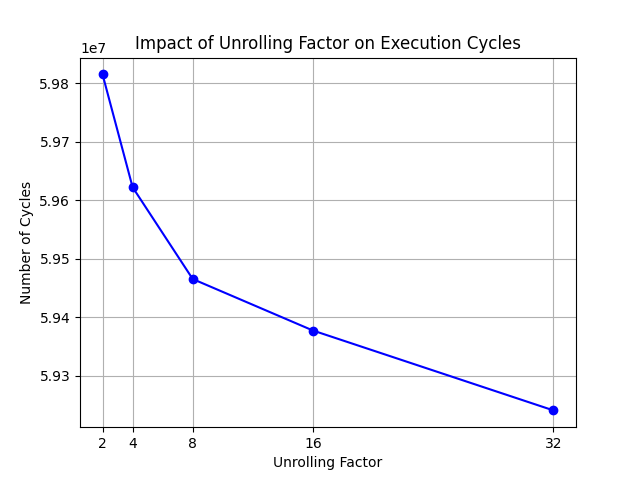
\includegraphics[width=0.8\linewidth]{unrolling_factors_plot.png}
\caption{Επίδραση του Unrolling Factor στον Χρόνο Εκτέλεσης}
\label{fig:LU}
\end{figure}

\subsection{Μέγεθος L1 Data Cache}
Συνεχίζοντας τη μελέτη της δεύτερης αρχιτεκτονικής, προχωράμε σε μια εξερεύνηση της επίδρασης διαφορετικών μεγεθών L1 Data Cache (2kB, 4 kB, 8kB, 16kB, 32kB και 64kB).

\begin{figure} [H]
\centering
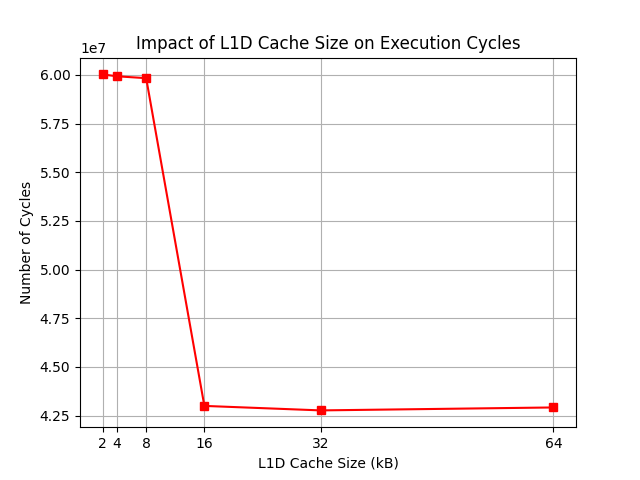
\includegraphics[width=0.8\linewidth]{l1d_cache_size_plot.png}
\caption{Επίδραση του Μεγέθους της L1 Data Cache στον Χρόνο Εκτέλεσης}
\label{fig:L1}
\end{figure}

Εδώ παρατηρούμε κάτι πολύ ενδιαφέρον...

\subsection{Βελτιστοποίηση με Εξαντλητική Αναζήτηση}
Έχοντας μελετήσει την επίδραση συγκεκριμένων παραμέτρων της εφαρμογής (Unrolling Factor) αλλά και της αρχιτεκτονικής (Μέγεθος L1 Data Cache), έχουμε σχηματίσει μια εικόνα για τη βελτιστοποίηση. Αυτό που μας ενδιαφέρει είναι να ελαχιστοποιήσουμε το πλήθος των κύκλων που απαιτούνται για την εκτέλεση της εφαρμογής αλλά και τη συνολική μνήμη που θα χρησιμοποιήσουμε (το άθροισμα των L1I, L1D και L2 σε kB). Έτσι, καταγράφουμε έναν χώρο προς εξερεύνηση, ο οποίος ορίζεται από τους συνδυασμούς των παρακάτω

\begin{center}
	\textbf{L1D Cache Size} $\in$ [2kB, 4kB, 8kB, 16kB, 32kB, 64kB] \\
	\textbf{L1I Cache Size} $\in$ [2kB, 4kB, 8kB, 16kB, 32kB, 64kB] \\
	\textbf{L2 Cache Size} $\in$ [128kB, 256kB, 512kB, 1024kB] \\
	\textbf{Unrolling Factor} $\in$ [2, 4, 8, 16, 32]
\end{center}

Προχωράμε σε εξαντλητική αναζήτηση του χώρου εξερεύνησης και για κάθε ένα από τα 720 σημεία του χώρου καταγράφουμε το πλήθος των κύκλων που απαιτούνται για την εκτέλεση της εφαρμογής. Στο Σχήμα \ref{fig:exhaustive-pf} φαίνονται οι θέσεις όλων των σημείων και το Pareto Frontier, ενώ στον Πίνακα \ref{tab:exhaustive-pf} παραθέτουμε το Pareto Frontier μαζί με τα στοιχεία της αρχιτεκτονικής που οδήγησαν στο εκάστοτε Pareto Optimal σημείο.

\begin{figure} [H]
\centering
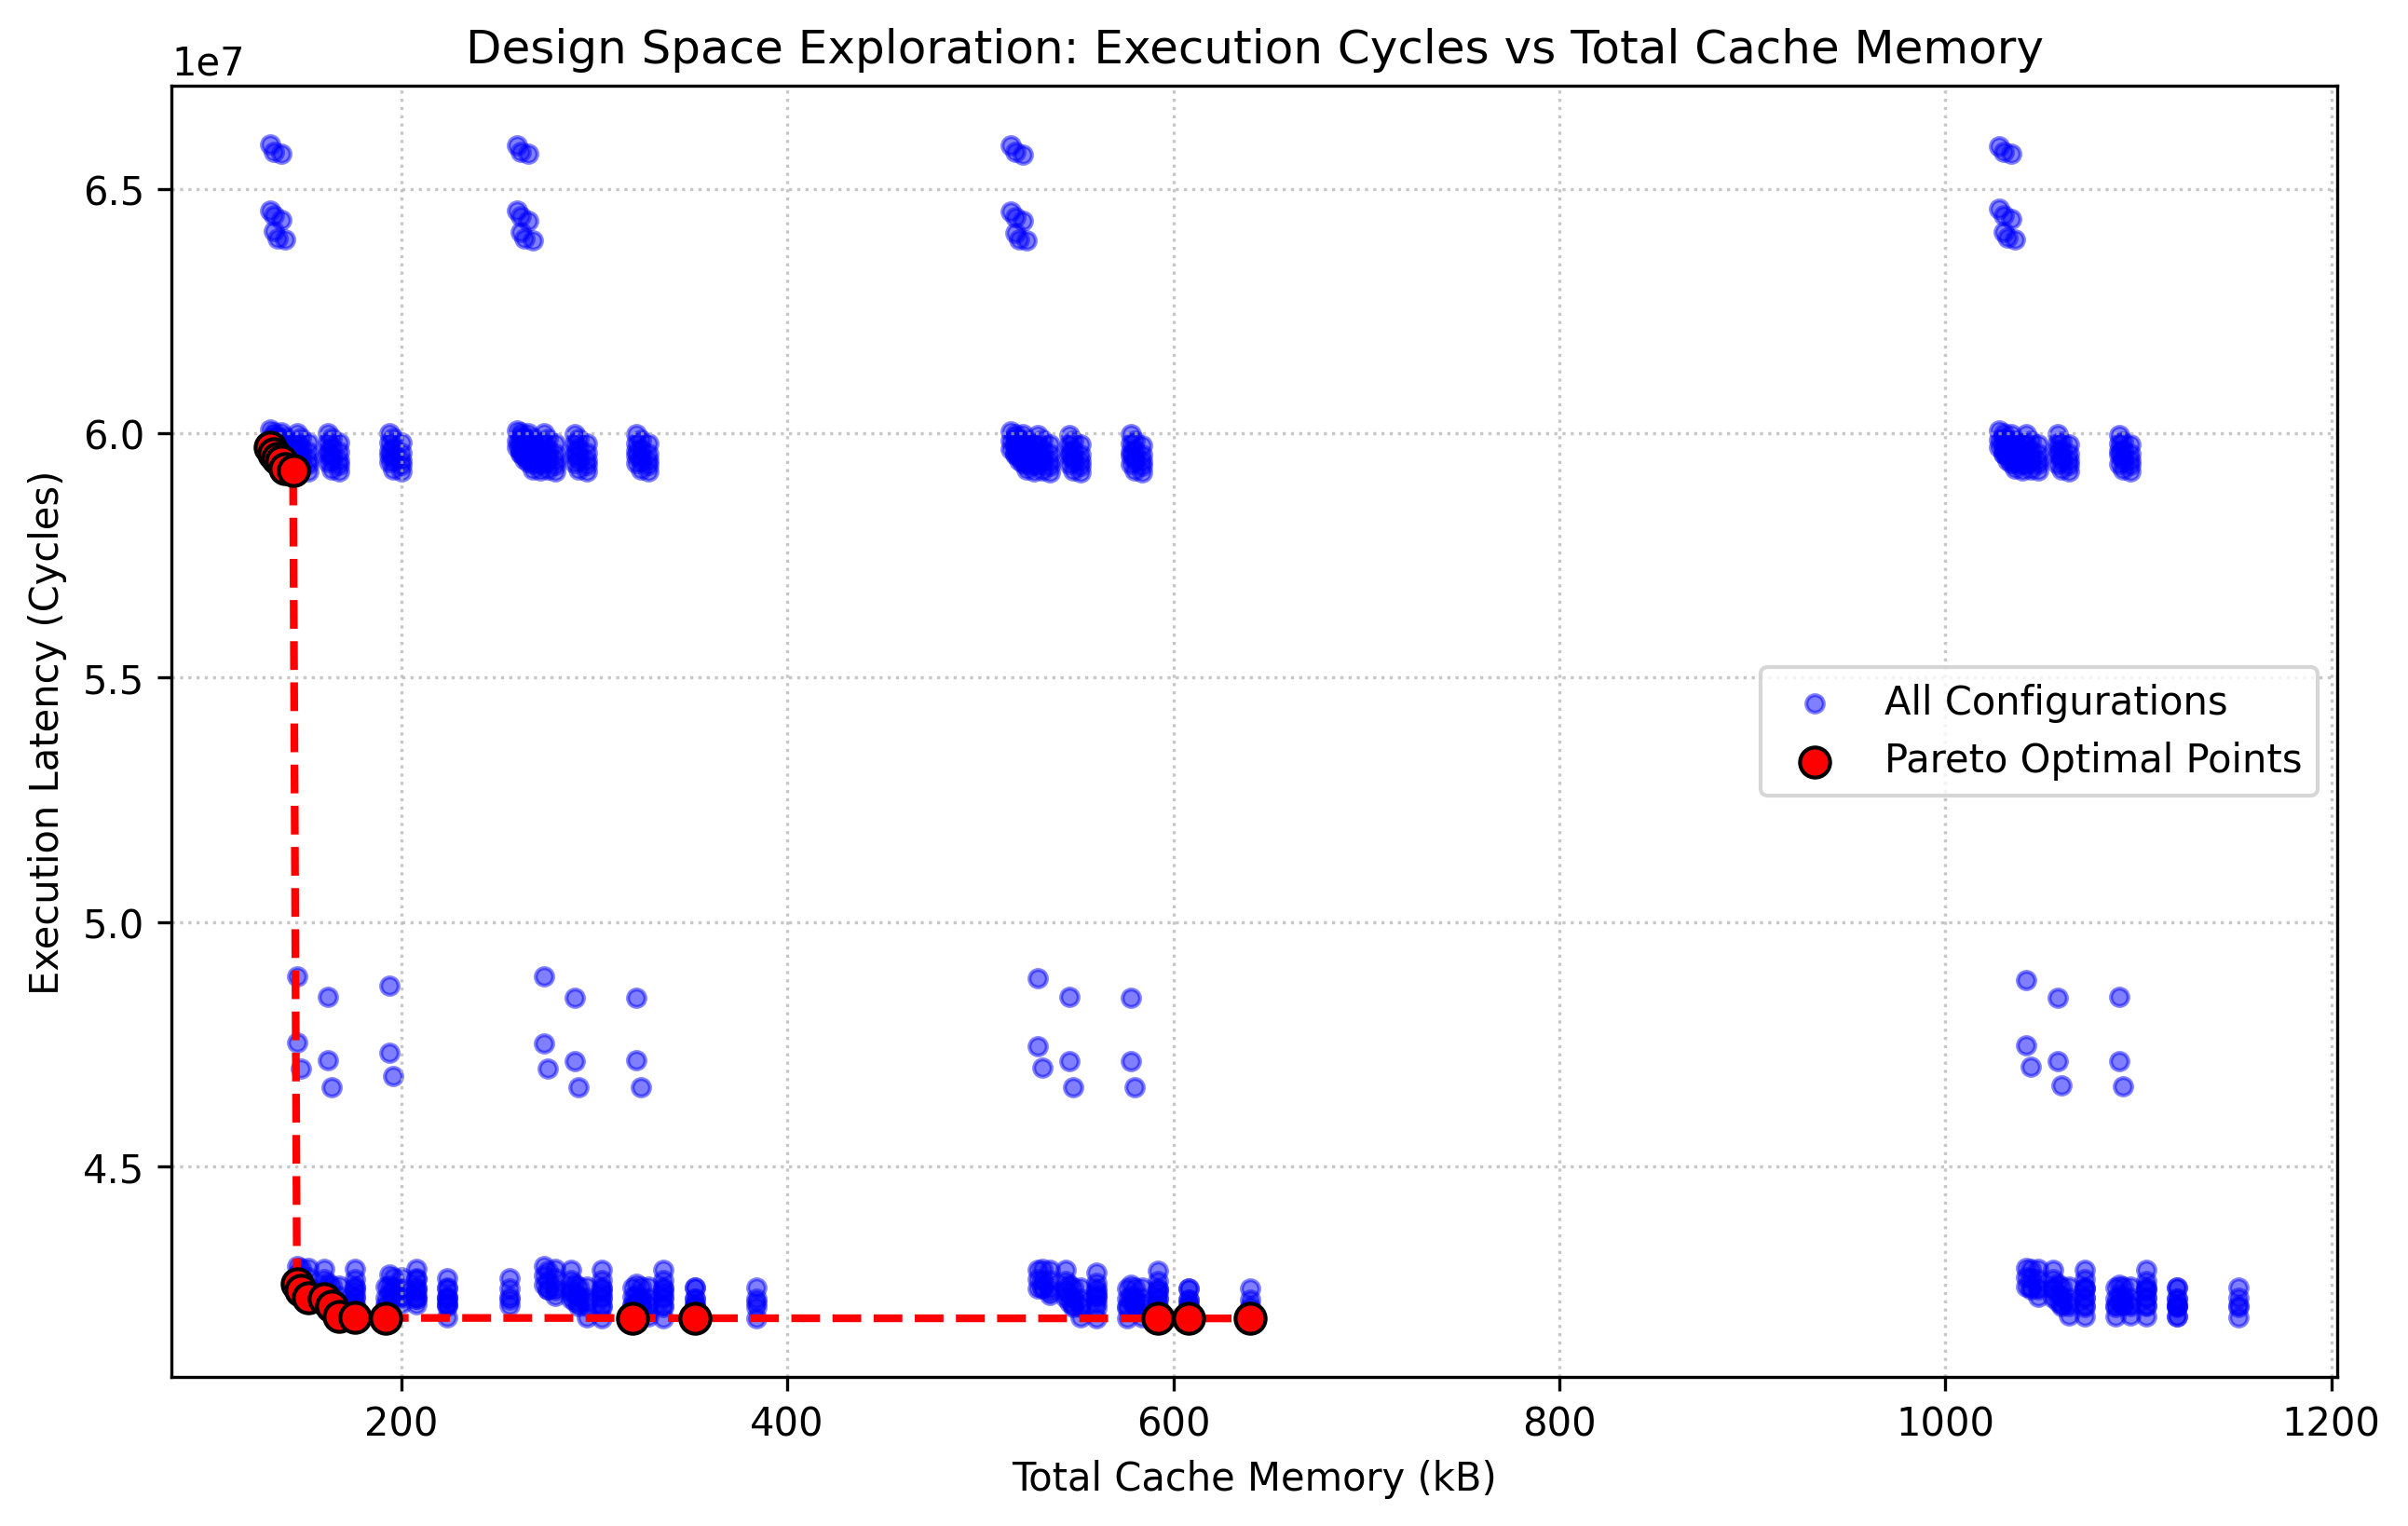
\includegraphics[width=0.8\linewidth]{pareto_frontier_plot.png}
\caption{Exhaustive Search Pareto Frontier}
\label{fig:exhaustive-pf}
\end{figure}

\begin{table}[H]
    \centering
    \csvreader[
        tabular=cccccc,
        table head=\toprule L1I (kB) & L1D (kB) & L2 (kB) & UF & Total Memory (kB) & Latency (CC) \\\midrule,
        table foot=\bottomrule,
        late after line=\\
    ]{pareto_frontier.csv}{}
    {\csvcoli & \csvcolii & \csvcoliii & \csvcoliv & \csvcolv & \csvcolvi}
    \caption{Exhaustive Search Pareto Optimal Points}
    \label{tab:exhaustive-pf}
\end{table}

Παρατηρούμε ότι... Τέλος, σημειώνουμε ότι λόγω του μεγάλου πλήθους προσομοιώσεων (720 σημεία), για την εξαντλητική αναζήτηση απαιτήθηκαν 2 ώρες και 46 λεπτά.

\subsection{Βελτιστοποίηση με τη χρήση Γενετικού Αλγορίθμου}
Αντί για τη χρονοβόρα εξαντλητική αναζήτηση του χώρου εξερεύνησης, μπορούμε να χρησιμοποιήσουμε έναν γενετικό αλγόριθμο για να λάβουμε το Pareto Frontier. Ο αλγόριθμος αυτός μπλα μπλα μπλα...

Εκτελώντας τον αλγόριθμο παρατηρούμε ότι κάνει μόνο 30 evaluations και τερματίζει σε 7 λεπτά και 30 δευτερόλεπτα, επιστρέφοντας το Pareto Frontier του Πίνακα \ref{tab:gen-pf}. Παρατηρούμε αρχικά ότι ο αλγόριθμος βρήκε 3 Pareto Optimal σημεία, σε αντίθεση με τα 19 της εξαντλητικής αναζήτησης. Τέλος, παρατηρούμε ότι μόνο ένα εκ των τριών σημείων (32kB, 32kB, 256kB, 32) είναι στην πραγματικότητα Pareto Optimal και βρίσκεται στα αποτελέσματα της προηγούμενης υποπαραγράφου. Αυτό συμβαίνει καθώς ο αλγόριθμος βασίζεται σε έναν ευρετικό (heuristic) μηχανισμό...

\begin{table}[H]
    \centering
    \csvreader[
        tabular=cccccc,
        table head=\toprule L1I (kB) & L1D (kB) & L2 (kB) & UF & Total Memory (kB) & Latency (CC) \\\midrule,
        table foot=\bottomrule,
        late after line=\\
    ]{genOptimizer_PO.csv}{}
    {\csvcoli & \csvcolii & \csvcoliii & \csvcoliv & \csvcolvi & \csvcolv}
    \caption{Genetic Algorithm Pareto Optimal Points}
    \label{tab:gen-pf}
\end{table}


\end{document}
